\documentclass[conference]{IEEEtran}
\IEEEoverridecommandlockouts
\usepackage{cite}
\usepackage{amsmath}
\usepackage{graphicx}
\usepackage{booktabs}
\usepackage{xcolor}
\usepackage{listings}
\usepackage{tikz}
\usetikzlibrary{positioning}
\usepackage{pgfplots}
\pgfplotsset{compat=1.18}
\usepackage[hidelinks]{hyperref}

\lstset{
    language=C++,
    morekeywords={import, export, module, concept, requires},
    basicstyle=\ttfamily\scriptsize,
    keywordstyle=\color{blue!60!black}\bfseries,
    commentstyle=\color{green!40!black},
    stringstyle=\color{red!50!black},
    columns=fullflexible,
    keepspaces=true,
    frame=single,
    framerule=0.3pt,
    xleftmargin=2pt,
    xrightmargin=2pt,
    aboveskip=6pt,
    belowskip=4pt,
}

\newcommand{\code}[1]{\texttt{#1}}
% Listings are kept in one piece, so a short listing is never split between columns.
\lstnewenvironment{codeblock}{\endgraf\noindent\minipage{\linewidth}}{\endminipage\endgraf}

\begin{document}

\title{Ember: A Minimalistic 2D Game Framework\\in Modern C++}

\author{
\IEEEauthorblockN{Roman Prokhorov}
\IEEEauthorblockA{\textit{Faculty of Applied Sciences} \\
\textit{Ukrainian Catholic University}\\
Lviv, Ukraine \\
prokhorov.pn@ucu.edu.ua}
\and
\IEEEauthorblockN{Kyrylo Omelianchuk}
\IEEEauthorblockA{\textit{Faculty of Applied Sciences} \\
\textit{Ukrainian Catholic University}\\
Lviv, Ukraine \\
omelianchuk.pn@ucu.edu.ua}
\and
\IEEEauthorblockN{Yurii Fito}
\IEEEauthorblockA{\textit{Faculty of Applied Sciences} \\
\textit{Ukrainian Catholic University}\\
Lviv, Ukraine \\
fito.pn@ucu.edu.ua}
\and
\IEEEauthorblockN{Solomiia Hadiichuk}
\IEEEauthorblockA{\textit{Faculty of Applied Sciences} \\
\textit{Ukrainian Catholic University}\\
Lviv, Ukraine \\
hadiichuk.pn@ucu.edu.ua}
}

\maketitle

\begin{abstract}
Ember is a minimalistic 2D game framework written in C++26. It is built from C++ modules
and follows the entity component system (ECS) pattern: game objects are entities, their data are components, and their behaviour is
written as systems that run in fixed stages of every frame. This report describes the
current state of the project. The ECS, the main loop with a fixed time step, the event
bus, logging, the platform layer over Raylib and a particle system simulated with
\code{std::simd} are implemented and covered by 134 unit tests. A sample game, Yozakura,
runs on these modules. Benchmarks show that the engine itself adds about 0.1~\textmu s
per frame and that one million particles are simulated in about 1~ms. Rendering, physics,
assets and debug tools are not implemented yet.
\end{abstract}

\begin{IEEEkeywords}
C++26, game engine, entity component system, C++ modules, SIMD, benchmarks
\end{IEEEkeywords}

\section{Introduction}

Ember is a 2D game framework for games written in C++. A game built with Ember consists of
entities with components and of systems that process these components every frame. The
engine provides the main loop, the scheduling of systems, communication between systems
through events, and access to the window, drawing, audio and input. The speed of these
parts is measured with benchmarks.

This report describes the current state of Ember. Section~II lists the tools,
Section~III the architecture, and Section~IV the modules that are implemented. Section~V shows the sample game, Section~VI the tests and Section~VII the
benchmarks. Section~VIII lists problems we met, and Section~IX the work that remains.

\section{Tools}

Ember is written in C++26 and built with GCC~16, CMake~4.2 and Ninja on Linux. Every engine
module is a C++ module, and the code uses \code{import std;} instead of standard headers.
CMake presets define a Debug and a Release build; one command,
\code{cmake --workflow --preset debug}, configures, builds and tests the project.

Other C++26 and C++23 features used in the code:
\begin{itemize}
    \item \code{std::simd}~\cite{simd} for the particle simulation;
    \item contracts~\cite{contracts}, which check preconditions of the engine API in Debug
          builds and are switched off in Release builds;
    \item \code{std::expected} for errors, for example when an image cannot be decoded;
    \item concepts, for example for plugins (Section~IV-B).
\end{itemize}

Windows, drawing, audio and input are provided by Raylib~6.0~\cite{raylib} through its
C++ wrapper raylib-cpp~\cite{raylibcpp}. Unit tests and benchmarks use Catch2~\cite{catch2}.
All warnings are enabled and treated as errors, and code is formatted with clang-format.
Two scripts help during development: \code{run.sh} builds and starts an example, and
\code{benchmark.sh} builds and runs the benchmarks.

\section{Architecture}

The engine is split into layers (Fig.~\ref{fig:layers}). A module may use only the
modules below it, so lower layers know nothing about higher ones:
\begin{itemize}
    \item \code{common}: math types (\code{Vec2}, \code{Rect}, \code{Color}) and typed
          handles;
    \item \code{ecs}: entities, components, views, resources and deferred commands;
    \item \code{core}: the application, the main loop, the scheduler, the event bus and
          logging;
    \item \emph{services}, modules that own resources and are called by other code:
          \code{platform}, \code{assets} and \code{debug};
    \item \emph{systems}, modules that run every frame over components: \code{physics},
          \code{particles} and \code{render}.
\end{itemize}
Services and systems do not depend on each other, except on \code{platform} for drawing
and audio. Only \code{platform} uses Raylib, and Raylib types never appear in exported
declarations. Thus the rest of the engine does not depend on the graphics library.

\begin{figure}[htbp]
\centering
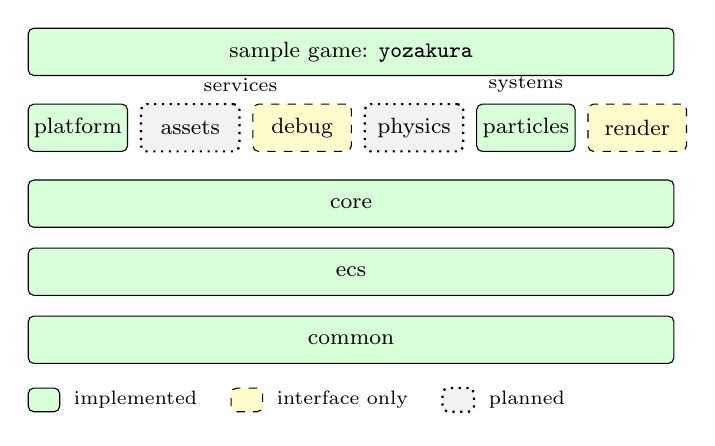
\begin{tikzpicture}[
    box/.style={draw, rounded corners=2pt, minimum height=0.6cm, align=center,
                font=\footnotesize, inner sep=2pt},
    done/.style={box, fill=green!15},
    iface/.style={box, fill=yellow!20, dashed},
    planned/.style={box, fill=gray!10, dotted, thick},
    node distance=0.25cm and 0.15cm]
    \node[done, minimum width=8.2cm] (game) {sample game: \code{yozakura}};
    \node[done, minimum width=1.25cm, below=0.35cm of game.south west, anchor=north west]
        (platform) {platform};
    \node[planned, minimum width=1.25cm, right=of platform] (assets) {assets};
    \node[iface, minimum width=1.25cm, right=of assets] (debug) {debug};
    \node[planned, minimum width=1.25cm, right=of debug] (physics) {physics};
    \node[done, minimum width=1.25cm, right=of physics] (particles) {particles};
    \node[iface, minimum width=1.25cm, right=of particles] (render) {render};
    \node[done, minimum width=8.2cm, below=0.35cm of platform.south west, anchor=north west]
        (core) {core};
    \node[done, minimum width=8.2cm, below=of core] (ecs) {ecs};
    \node[done, minimum width=8.2cm, below=of ecs] (common) {common};
    \node[font=\scriptsize, above=0.02cm of assets.north east] {services};
    \node[font=\scriptsize, above=0.02cm of particles.north] {systems};
    \node[done, minimum width=0.4cm, minimum height=0.3cm, below=0.3cm of common.south west,
          anchor=north west] (k1) {};
    \node[font=\scriptsize, right=0.05cm of k1] (l1) {implemented};
    \node[iface, minimum width=0.4cm, minimum height=0.3cm, right=0.3cm of l1] (k2) {};
    \node[font=\scriptsize, right=0.05cm of k2] (l2) {interface only};
    \node[planned, minimum width=0.4cm, minimum height=0.3cm, right=0.3cm of l2] (k3) {};
    \node[font=\scriptsize, right=0.05cm of k3] {planned};
\end{tikzpicture}
\caption{Layers of Ember and the state of each module. A module uses only the layers
below it.}
\label{fig:layers}
\end{figure}

\section{Implemented Modules}

\subsection{Entity Component System}

An entity is a pair of an index and a generation. When an entity is destroyed, its index
can be given to a new entity, but with a higher generation. An old copy of the entity then
no longer matches, so it cannot read the components of the new entity by mistake.

Components of one type are kept in a \emph{sparse set}~\cite{entt}: a dense array of
components without holes and a sparse array that maps an entity index to a position in
the dense array. Adding, finding and removing a component take constant time, and
iteration goes over a packed array. When a component is removed, the last component is
moved into its place, so the array stays packed.

A \emph{view} iterates over all entities that have a given set of components and is used
with structured bindings:
\begin{codeblock}
for (auto [entity, player, transform] :
     world.view<Player, const Transform>())
\end{codeblock}
A system that iterates a view must not create or destroy entities. It records these
changes as \emph{commands}, and the world applies them later. \emph{Resources} are single
objects of a type stored in the world, such as the window or the game settings. The ECS
also defines the components shared by all modules: \code{Transform}, \code{Velocity},
\code{Collider}, \code{RigidBody}, \code{Sprite}, \code{Camera}, \code{Emitter} and
\code{Name}.

\subsection{Core: Application, Stages and Main Loop}

A game creates an \code{Application}, adds plugins and its own systems, and calls
\code{run()}. A plugin is any type with a \code{build} function, similar to the plugins
of Bevy~\cite{bevy}. Usually one module provides one plugin, and its fields are the
settings of the module.

\begin{codeblock}
template <typename P>
concept Plugin = requires(const P& plugin,
                          Application& app) {
    plugin.build(app);
};
\end{codeblock}

A system is a function that receives the world. Every system is added to one of nine
stages, which run in this order every frame:
\code{Startup} (first frame only), \code{PreUpdate}, \code{FixedUpdate},
\code{Update}, \code{PostUpdate}, \code{PreRender}, \code{Render}, \code{PostRender}, and
\code{Shutdown} (after the last frame). Inside a stage the systems run in the order they
were added. After every stage the scheduler applies the recorded commands. If a system
throws an exception, the scheduler logs the name of the system and passes the exception on.

\code{FixedUpdate} runs with a fixed time step, by default 1/60~s, which makes movement
the same on fast and slow computers~\cite{fiedler}. The time of each frame is added to an
accumulator, and \code{FixedUpdate} runs once for every full step in it, from zero to five
times per frame. The time that is left, divided by the step, is stored as
\code{fixed\_alpha}, which can be used to draw objects between two steps. Very long frames,
for example after a breakpoint, are treated as 0.25~s long.

The \emph{event bus} lets systems talk without knowing each other. An event published in
one frame can be read by all systems in the next frame. Each event type has its own
channel with two lists, one for publishing and one for reading, which are swapped at the
start of a frame. Publishing takes a lock, so it is safe from several threads. For
example, closing the window publishes \code{ExitRequested}, and the application stops
after the next frame.

\emph{Logging} has five levels and a list of outputs (sinks). Messages are formatted with
\code{std::format} only if their level is enabled.

\subsection{Platform}

The \code{platform} module wraps Raylib and provides five services, stored as resources:
\code{Window}, \code{Graphics} (textures, fonts, shapes, a camera view),
\code{Input} (keys and mouse, with named actions such as \code{"jump"} that can be
bound to several keys), \code{Audio} (sounds and music) and image decoding. Textures,
fonts and sounds are loaded from bytes in memory and returned as typed handles. A handle
uses the same index and generation idea as an entity, so a handle to an unloaded texture
is detected and ignored. The \code{PlatformPlugin} adds systems that read input and
begin and end the frame of drawing.

\subsection{Particles}

An \code{Emitter} component describes particles: how many per second, their lifetime,
speed, direction, acceleration (for example gravity), and start and end color and size.
Each emitter has its own \emph{pool} of particles with a fixed capacity, by default 1024.
The pool is a \emph{structure of arrays}: positions, velocities and ages are kept in
separate \code{float} arrays. Thus several particles can be loaded into one SIMD register
and updated by one instruction, as in the shortened loop below. On our computers a
register holds four floats. The particles left over at the end, fewer than one register,
are updated by normal scalar code.

\begin{codeblock}
using FloatVector = std::simd::vec<float>;
auto vx = unchecked_load<FloatVector>(chunk(m_velocity_x));
auto px = unchecked_load<FloatVector>(chunk(m_position_x));
// ... the same for y and the age
vx += velocity_change.x;
px += vx * dt;
age += dt;
unchecked_store(vx, chunk(m_velocity_x));
unchecked_store(px, chunk(m_position_x));
\end{codeblock}

The pool also has a plain scalar version of the same loop. A unit test checks that both
versions give the same results, and the benchmarks compare their speed. Dead particles
are removed by moving the last particle into their place, because the order of particles
does not matter. The \code{ParticlePlugin} simulates all emitters in \code{Update} and
draws the particles as squares in \code{Render}.

\section{Sample Game: Yozakura}

Yozakura (Fig.~\ref{fig:game}) is a small game that tests the engine as a whole. The
player controls a girl under a cherry tree at night and catches falling spirits. A missed
spirit costs one of three lives, and golden spirits give more points. The girl can run,
jump and dash. The game becomes faster over time and shows the best score of the session.

\begin{figure}[htbp]
\centerline{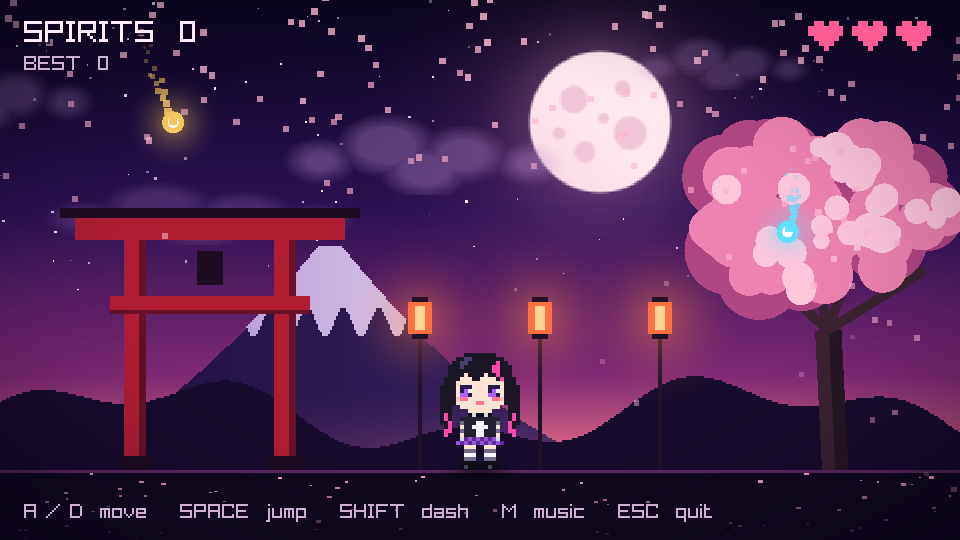
\includegraphics[width=\columnwidth]{figures/yozakura.png}}
\caption{The sample game Yozakura. The falling petals and the flames of the spirits are
drawn by the particle system.}
\label{fig:game}
\end{figure}

The game has no asset files. Because the \code{assets} module is not ready, all images
are drawn pixel by pixel in code, and all sounds and the music are computed as waves and
packed into WAV files in memory. They are loaded through the same \code{platform}
functions that would load real files. The game is about 2100 lines in three modules.
Its \code{main} function shows how a game uses the engine:
\begin{codeblock}
Application app;
app.add_plugin(platform::PlatformPlugin{...});
app.add_system(Stage::FixedUpdate, "move_player",
               move_player);
app.add_system(Stage::Update, "catch_spirits",
               catch_spirits);
// ... ten more systems
app.add_plugin(particles::ParticlePlugin{});
app.run();
\end{codeblock}

\section{Testing}

Every implemented module has unit tests (Table~\ref{tab:tests}). Tests run in both
builds: in Debug the contracts are checked as well. Tests that need a window or an audio
device are skipped on a computer without them. All 134 test cases pass.

\begin{table}[htbp]
\caption{Unit Tests per Module}
\label{tab:tests}
\centering
\footnotesize
\begin{tabular}{@{}lr@{}}
\toprule
\textbf{Module} & \textbf{Test cases} \\
\midrule
\code{ecs} & 39 \\
\code{core} & 45 \\
\code{platform} & 22 \\
\code{particles} & 28 \\
\midrule
Total & 134 \\
\bottomrule
\end{tabular}
\end{table}

\section{Benchmarks}

Benchmarks use the \code{BENCHMARK} macro of Catch2, which runs code many times and
reports the mean time. They were run on a laptop with an Intel Core i7-13700H in the
Release build (\code{-O3}).

\subsection{Particles: SIMD and Scalar Code}

Table~\ref{tab:particles} shows the time to simulate one step of a full pool. The SIMD and
the scalar versions take almost the same time. The reason is that GCC
\emph{auto-vectorizes} the scalar loop: at \code{-O3} it turns the simple loop into SIMD
code by itself.

\begin{table}[htbp]
\caption{One Simulation Step of a Particle Pool}
\label{tab:particles}
\centering
\footnotesize
\begin{tabular}{@{}rrr@{}}
\toprule
\textbf{Particles} & \textbf{SIMD} & \textbf{Scalar} \\
\midrule
1\,000 & 0.60~\textmu s & 0.61~\textmu s \\
10\,000 & 7.0~\textmu s & 6.5~\textmu s \\
100\,000 & 74~\textmu s & 70~\textmu s \\
1\,000\,000 & 1.06~ms & 1.03~ms \\
\bottomrule
\end{tabular}
\end{table}

To check this, we built the benchmarks again with auto-vectorization switched off
(\code{-fno-tree-vectorize}) and also with AVX2 instructions (\code{-march=native}).
Fig.~\ref{fig:vectorize} shows the results for 100\,000 particles. Without
auto-vectorization the scalar code is about two times slower, while the \code{std::simd}
code keeps its speed. AVX2 registers hold eight floats instead of four, but they did not
make the code faster. We think the limit here is the speed of memory, not of the
arithmetic, because the loop does little work for every float it reads.

\begin{figure}[htbp]
\centering
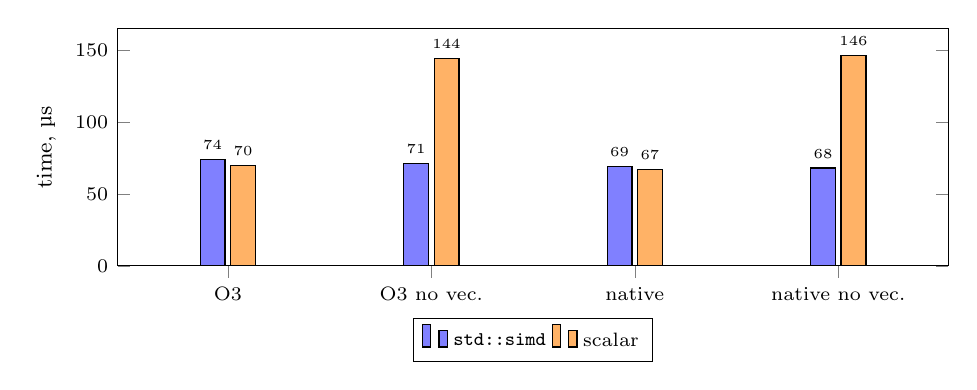
\begin{tikzpicture}
\begin{axis}[
    width=\columnwidth, height=4.6cm,
    ybar, bar width=9pt,
    ymin=0, ymax=165,
    ylabel={time, \textmu s}, ylabel style={font=\footnotesize},
    symbolic x coords={O3, O3 no vec., native, native no vec.},
    xtick=data,
    xticklabel style={font=\scriptsize},
    yticklabel style={font=\scriptsize},
    nodes near coords, nodes near coords style={font=\tiny},
    xtick pos=bottom,
    legend columns=2,
    legend style={font=\scriptsize, at={(0.5,-0.22)}, anchor=north},
    enlarge x limits=0.18,
]
\addplot[fill=blue!50] coordinates
    {(O3,74) (O3 no vec.,71) (native,69) (native no vec.,68)};
\addplot[fill=orange!60] coordinates
    {(O3,70) (O3 no vec.,144) (native,67) (native no vec.,146)};
\legend{\code{std::simd}, scalar}
\end{axis}
\end{tikzpicture}
\caption{One step of 100\,000 particles with different compiler options. ``No vec.''
means that auto-vectorization is switched off.}
\label{fig:vectorize}
\end{figure}

So explicit \code{std::simd} code gives the same speed as the best compiler output, and
it does not depend on whether the compiler manages to vectorize the loop. A small change
in the loop can stop auto-vectorization without any warning, while explicit SIMD code
stays vectorized.

Other results for particles: emitting a burst of 100\,000 particles with random speed and
direction takes 1.09~ms. A full frame of the particle plugin takes 11~\textmu s for
10~emitters (10\,240 particles), 110~\textmu s for 100~emitters, and 1.5--1.8~ms for
1000~emitters (about one million particles). At 60 frames per second a frame lasts
16.7~ms, so even one million particles use about a tenth of it. Drawing the particles is
not measured yet.

\subsection{Core}

Table~\ref{tab:core} shows the cost of the main parts of \code{core}. A frame of an
application without systems takes about 0.1~\textmu s, and the scheduler adds less than
one nanosecond per system. A log message below the enabled level costs 0.4~ns, so debug
messages can stay in the code. Events are the most expensive part, about 17~ns per event,
mostly because of the lock in \code{publish}.

\begin{table}[htbp]
\caption{Overhead of the Core Module}
\label{tab:core}
\centering
\footnotesize
\begin{tabular}{@{}lr@{}}
\toprule
\textbf{Operation} & \textbf{Time} \\
\midrule
Filtered-out \code{log\_debug} call & 0.4~ns \\
Stage with 1 / 10 / 100 empty systems & 2.6 / 12 / 90~ns \\
One step of the fixed time step & 7.8~ns \\
Application frame without systems & 99~ns \\
Publish and read one event & 63~ns \\
Publish and read 10\,000 events & 175~\textmu s \\
\bottomrule
\end{tabular}
\end{table}

\section{Problems We Met}

C++26 support in GCC~16 is new, and we met several problems:
\begin{itemize}
    \item \code{import std;} does not provide \code{std::simd} yet, so the particle module
          includes the \code{<simd>} header in its global module fragment.
    \item \code{partial\_store} of \code{std::simd} wrote short chunks incorrectly, so the
          SIMD loop handles only full registers and leaves the rest to scalar code.
    \item The compiler crashed (an internal compiler error) on one \code{std::memcpy} call
          in the Release build; we replaced it with a vector constructor.
    \item Raylib crashed when it was given invalid font data, so \code{platform} checks the
          tables of a font file before passing it to Raylib.
\end{itemize}

\section{Current State and Future Work}

The base of the engine works: \code{ecs}, \code{core}, \code{platform} and
\code{particles} are implemented and tested, and the sample game runs on them. The
following work remains:
\begin{itemize}
    \item \code{render}: drawing \code{Sprite} components with a camera, culling and
          layers. Its interface is written; today the game draws its scene itself.
    \item \code{debug}: an in-game overlay, a console and an entity inspector. Its
          interface is written.
    \item \code{physics}: rigid bodies, box and circle colliders and collision events.
          Today the game moves its objects in its own systems.
    \item \code{assets}: assets built into the executable with \code{\#embed}, and
          loading and saving of scenes.
    \item Reflection helpers, which convert components to and from JSON with C++26
          reflection, and the component registry that uses them. Their interfaces are
          written.
    \item A parallel scheduler with \code{std::execution}: systems will declare which
          components they read and write, and systems that do not conflict will run at
          the same time.
    \item Benchmarks of ECS iteration, physics and drawing.
\end{itemize}

\section{Conclusion}

Ember shows that a small game framework can be built with C++26 modules and the newest
standard library features on the current GCC. The ECS, the main loop, the event bus, the
platform layer and the particle system work together in a playable game and are covered by
134 unit tests. The benchmarks show that the cost of the engine itself is very small and
that explicit SIMD code keeps the particle simulation fast regardless of compiler options.
The next steps are the remaining modules and parallel execution of systems.

\section*{Acknowledgment}

The authors thank their mentor Oles-Volodymyr Yarish for guidance and feedback on the
project.

\begin{thebibliography}{00}
\bibitem{raylib} R. Santamaria, ``raylib: a simple and easy-to-use library to enjoy
videogames programming.'' [Online]. Available: \url{https://www.raylib.com}
\bibitem{raylibcpp} R. Loach, ``raylib-cpp: C++ object oriented wrapper for raylib.''
[Online]. Available: \url{https://github.com/RobLoach/raylib-cpp}
\bibitem{catch2} ``Catch2: a modern, C++-native test framework for unit-tests, TDD and
BDD.'' [Online]. Available: \url{https://github.com/catchorg/Catch2}
\bibitem{simd} M. Kretz, ``std::simd --- merge data-parallel types from the Parallelism
TS~2,'' ISO/IEC JTC1/SC22/WG21, P1928.
\bibitem{contracts} J. Berne, T. Doumler, and A. Krzemie\'nski, ``Contracts for C++,''
ISO/IEC JTC1/SC22/WG21, P2900.
\bibitem{entt} M. Caini, ``EnTT: a fast and reliable entity component system.''
[Online]. Available: \url{https://github.com/skypjack/entt}
\bibitem{bevy} ``Bevy: a refreshingly simple data-driven game engine built in Rust.''
[Online]. Available: \url{https://bevyengine.org}
\bibitem{fiedler} G. Fiedler, ``Fix your timestep!'' Gaffer On Games, 2004. [Online].
Available: \url{https://gafferongames.com/post/fix_your_timestep/}
\end{thebibliography}

\end{document}
